\section{Method}

This section covers the choices made during the design of \acrshort{vcu20}. Each subsection takes on a different challenge encountered in the 2019 season, see section \ref{sec:2019sys}.

\subsection{System-on-Module}

The Zynq-7000 platform provided a sufficient platform for running the \acrshort{tv} algorithm and control loop. However, the Zynq-7000 \acrshort{soc} product line are only available in \acrshort{bga} packages. This introduced unwanted complexity to the design, both in term of requirements to the \acrshort{pcb} manufacturing, and to the assembly of the circuit boards which is a process that normally is performed by team members at the electronic workshop at Revolve NTNU's headquarters. 

In regards to the \acrshort{pcb} production process, the \acrshort{bga} package of the \acrshort{soc} adds two kinds of complexity to the design. The first is the need for very tight tolerances. To be able to properly extract all necessary signals from the \acrshort{soc}, a trace width of $0.1\si{\milli\metre}$ is needed. Secondly, the circuit board requires a higher number of layers. This is mainly because the \acrshort{soc} requires multiple different supply voltages, $1\si{\volt}$, $1.8\si{\volt}$ and $3.3\si{\volt}$ in the case of Z-7010, the specific \acrshort{soc} utilized in \acrshort{vcu19}. 

Both these requirements increase the price of \acrshort{pcb} production drastically. Although \acrshort{pcb} production houses have increased in number over the last few years, thereby driving the manufacturing cost down, special production techniques like more than 4 layer \acrshort{pcb}s and $0.1\si{\milli\metre}$ trace widths still introduces high costs to production runs. Table \ref{tab:pcb_cost} shows a cost comparison of the different tolerances and layer numbers. 

\begin{table}[H]
    \centering
    \caption{Prototype \acrshort{pcb} production cost depending on tolerance and number of layers. Data gathered from PCBWay's online instant quotation tool\cite{pcbway}.}
    \begin{tabular}{llll}
        \toprule
        Layers & Tolerance & Quantity & Cost \\
        \midrule
        4 & 0.20\si{\milli\metre} & 5 & 49 USD \\
        8 & 0.10\si{\milli\metre} & 5 & 388 USD \\
        \bottomrule
    \end{tabular}
    \label{tab:pcb_cost}
\end{table}
 
 
The solution to this issue is to employ as System-on-Module. Instead of mounting the SoC directly on the VCU20 PCB, we can purchase off-the-shelf SoC modules. These modules consists of a small PCB featuring a SoC and some peripherals like external DDR RAM and non-volatile flash memory. The modules interconnects with the VCU PCB by one or more PCB connectors which are easier to route. The downsides to using these modules is mainly the cost. The module utilized for VCU20, Enclustra Mercury ZX5 with Zynq-7015 (figure \ref{fig:zx5}), has a unit price of 318USD. However, as they are modular, they can easily be reused between seasons. Reusing soldered ICs is not common practice at Revolve NTNU, so this should mitigate the high entry cost at least to some extent.

\begin{figure}[H]
    \centering
    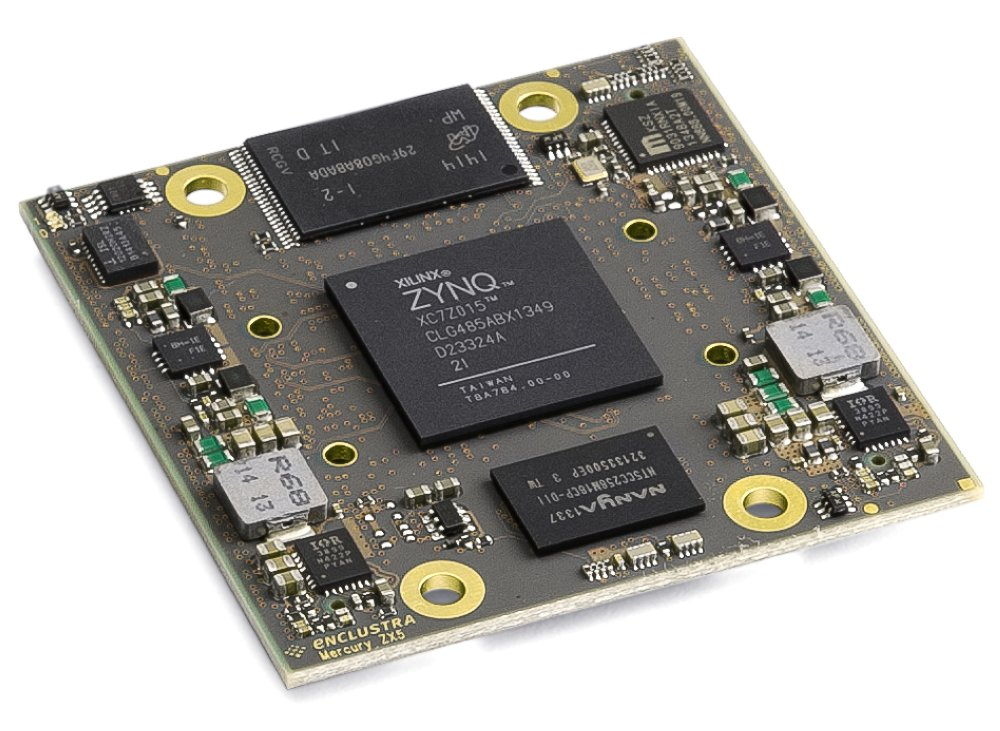
\includegraphics[width=.75\textwidth]{media/zx5.jpg}
    \caption{Enclustra Mercury ZX5 \acrshort{som}. Product image retrieved from Enclustra website \cite{zx5_img}.}
    \label{fig:zx5}
\end{figure}

%but at the cost of high design complexity. By utilizing a Zynq-7000 based System-on-Module (SoM), we avoid the hard parts of PCB layout, and simply design the VCU as a \emph{breakout board} for the SoM. Using a SoM also gives us access to peripherals that would have been difficult to implement by ourselves, specifically Ethernet, external flash memory and external double data-rate (DDR) memory.


\subsection{Partitioning interfaces}

As the VCU is an integral part of the EV, issues regarding the vehicle are also issues for the VCU. This section is dedicated to some of the issues encountered during last season, which hopefully can be solved by improving the design of the VCU.


In Nova, the main communication channel for the embedded systems were two CAN-FD buses running at a base frequency of 1MHz and an data transfer frequency of 4MHz. A system overview can be seen in figure \ref{fig:vcu19_system}.

\begin{figure}[H]
    \centering
    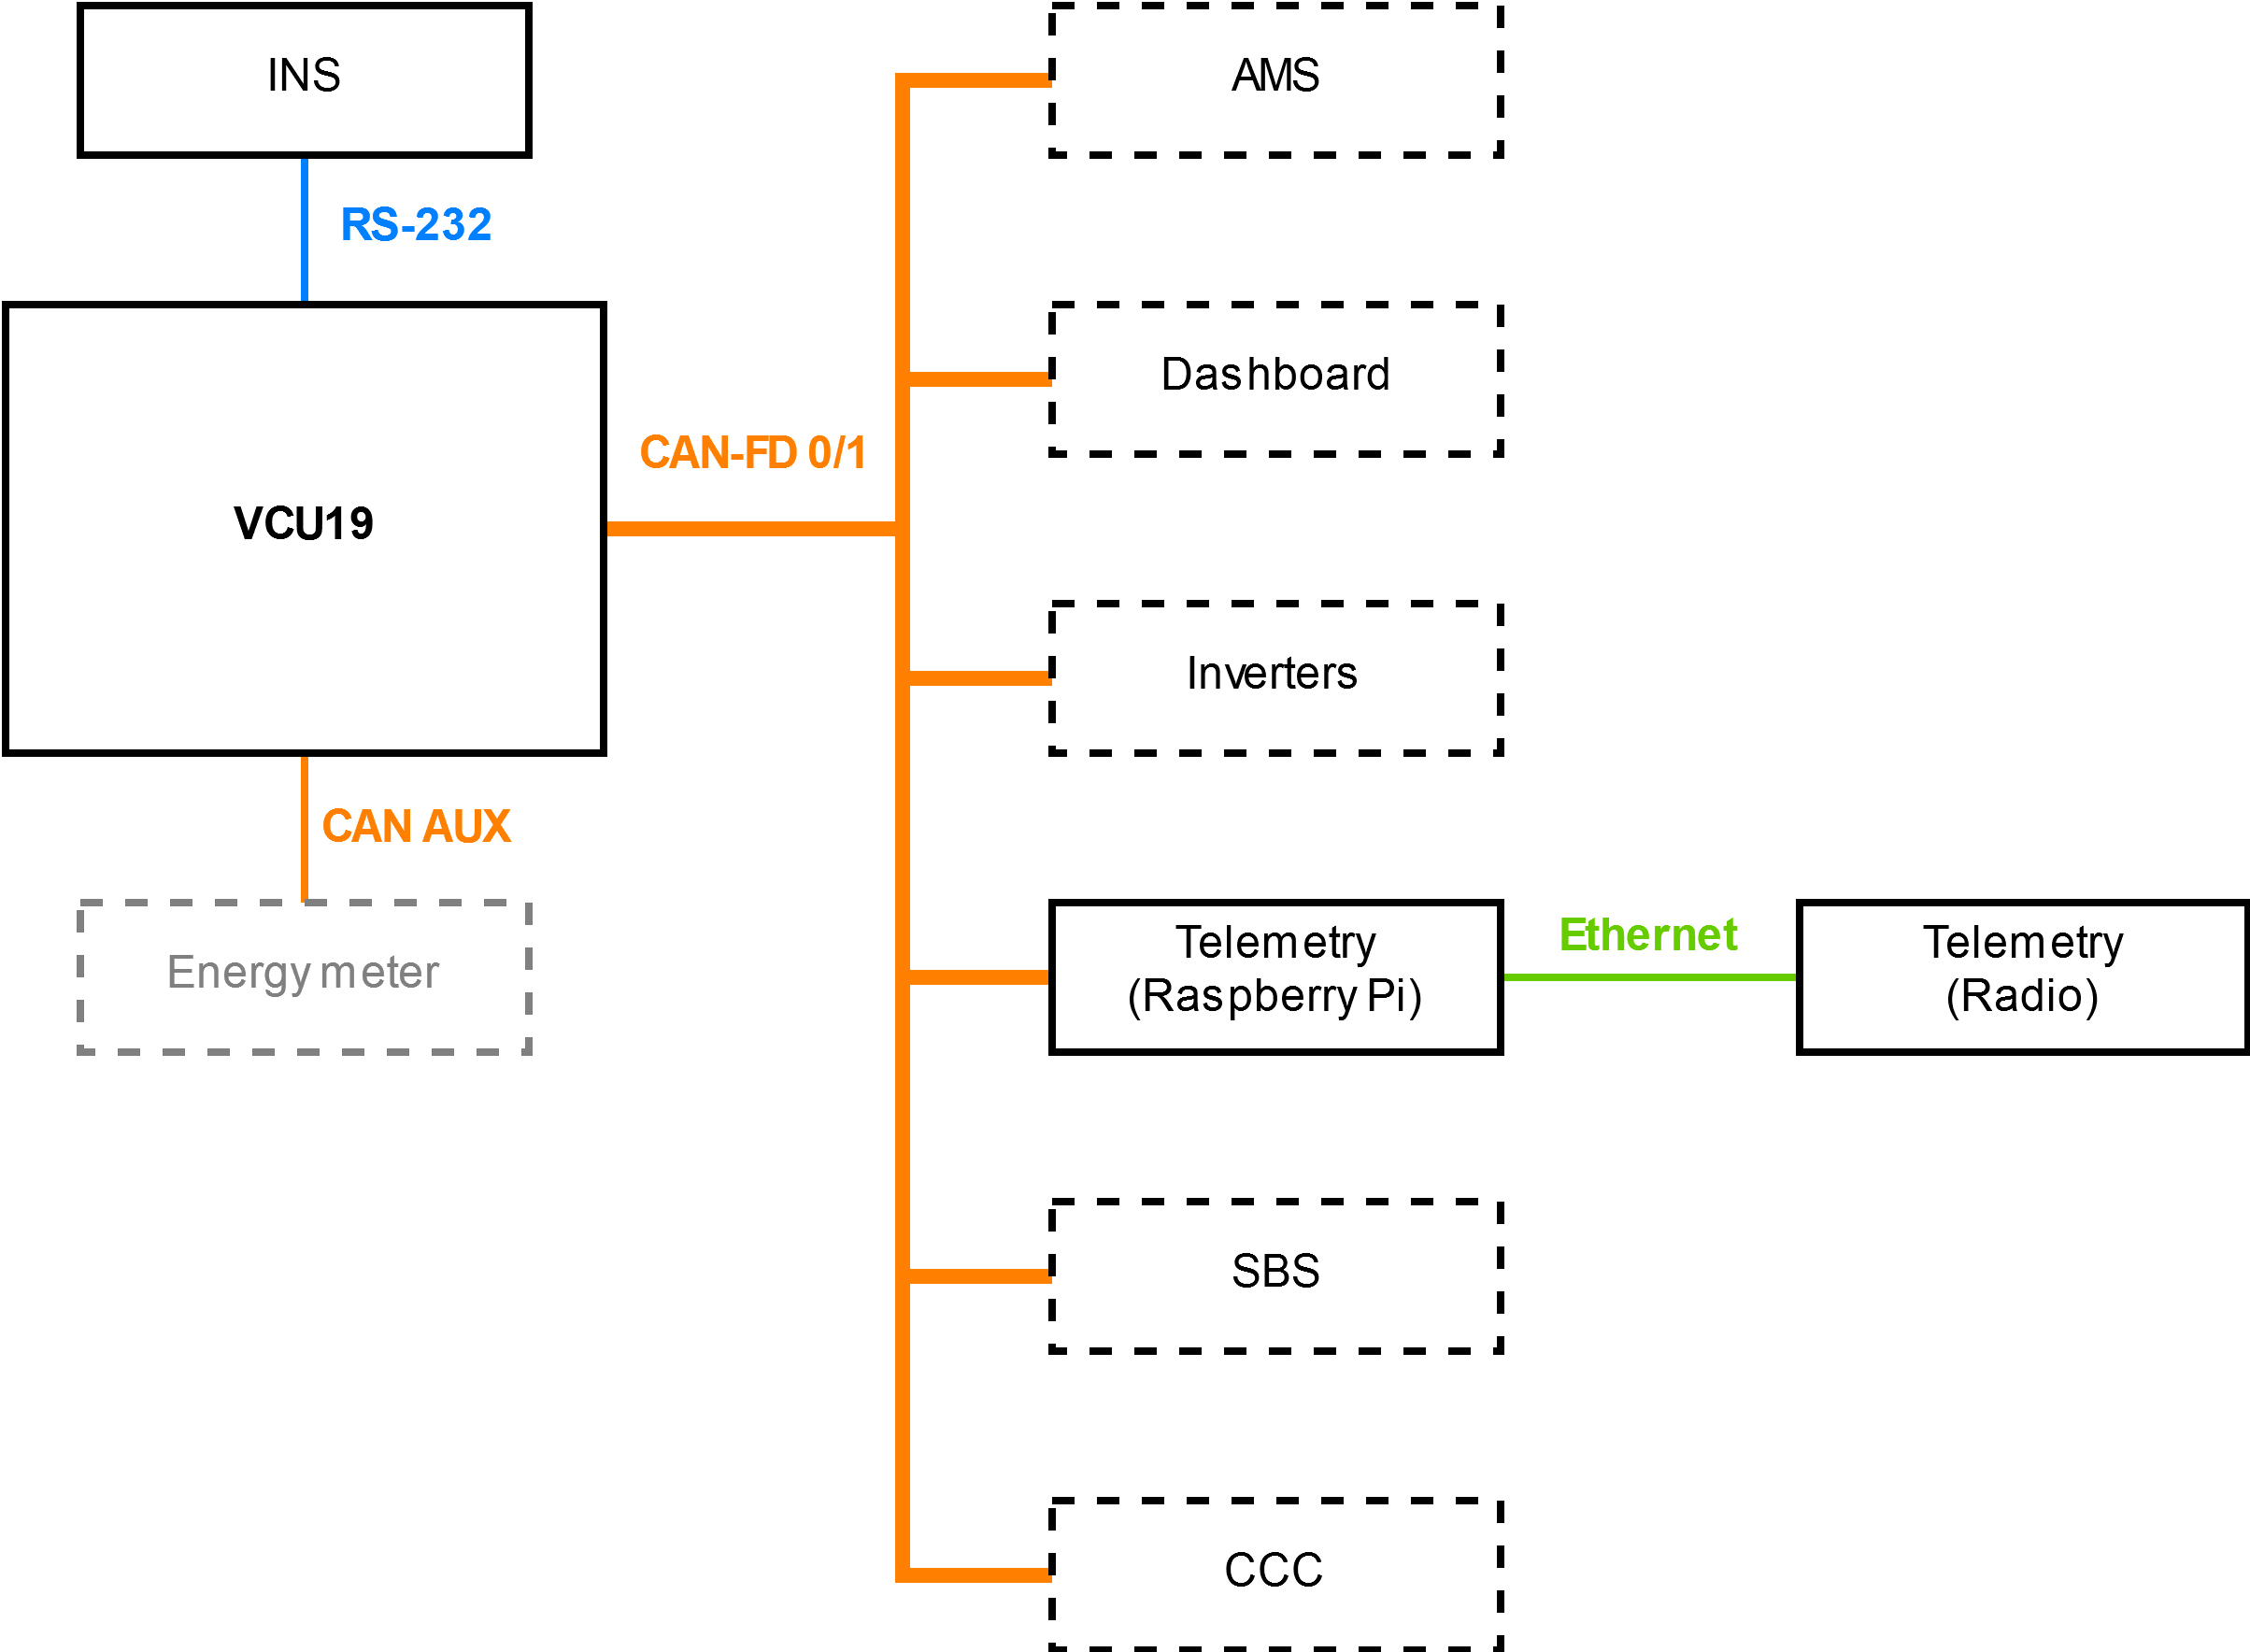
\includegraphics[width=.85\textwidth]{media/vcu19_system.png}
    \caption{VCU19 interface overview. Systems developed by other team members have dotted borders.}
    \label{fig:vcu19_system}
\end{figure}

There are several points where this system can be improved. They will be discussed in detail in the following subsections.


\subsubsection{CAN-FD buses}

A trace of the load on both CAN-FD buses during normal operation can be seen in figure \ref{fig:canfd_load}. Note the increase in load on bus 1 halfway into the trace. This is caused by the car entering \acrfull{de} mode where the \acrshort{vcu} starts transmitting set points to the inverters. 

\begin{figure}[H]
    \centering
    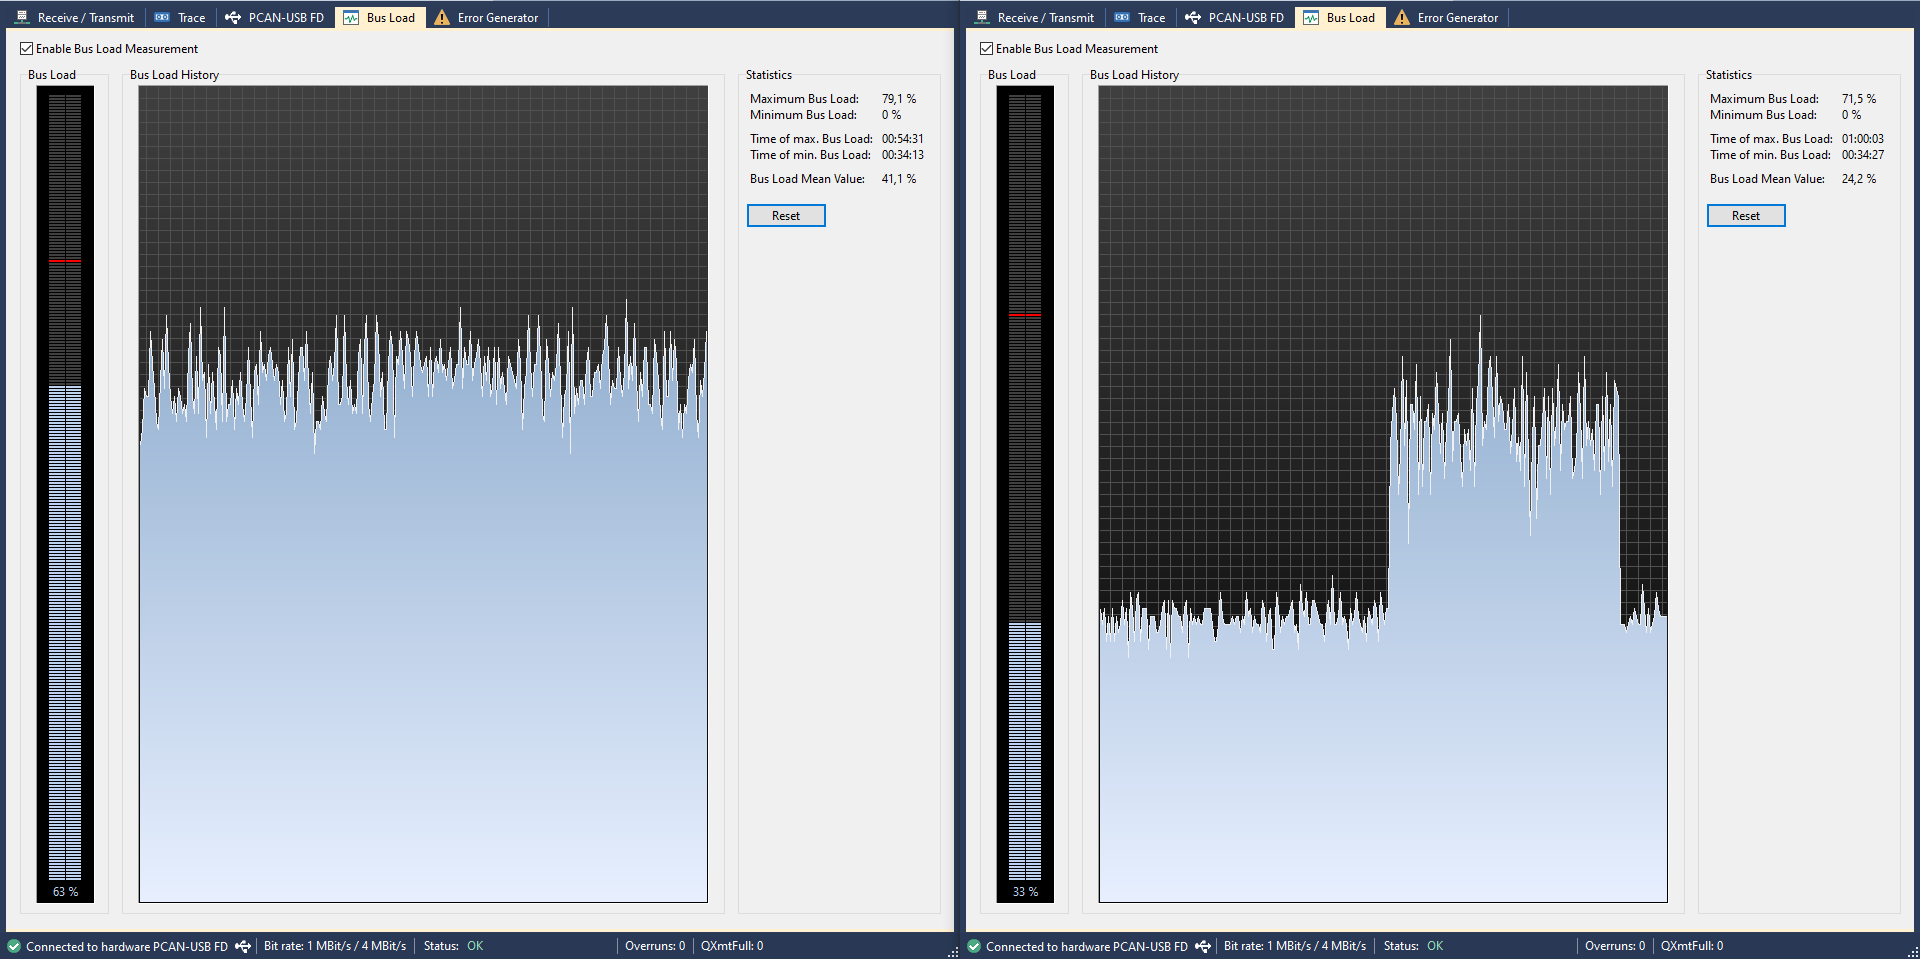
\includegraphics[width=\textwidth]{media/canfd-load.png}
    \caption{CAN-FD bus load in Nova during normal operation, screendumps from PCAN-View \cite{pcanview}. Vertical axis is utilization and horizontal axis is time. Utilization scale goes from 0\% to 100\%. Bus 0 on the left and bus 1 on the right.}
    \label{fig:canfd_load}
\end{figure}

From the traces we can see that bus 0 typically has a utilization of 60-70\% while bus 1 rests at about 30\% while out of \acrshort{de} mode and around 60\% in \acrshort{de} mode. This seems to be within the maximum utilization of 69\%, calculated in section \ref{sec:max_util}.

we know that to ensure that no frames are dropped (i.e. all deadlines are met) the bus utilization should be no more than 69\%. For bus 1, this seems to be in order. The trace tells us that the peak utilization is 71.3\%, but this is an outlier and probably not an issue. However, bus 0 seems to have a somewhat high bus load continuously, staying around 70\% load with peaks as high as 79.1\%. This is an area that can be improved.

To start of, we will take a closer look at the frames that are transmitted on each bus. Last season, the team started the process of transitioning from an in-house protocol on top of CAN/CAN-FD (called the Revolve Protocol), to a standardized alternative, UAVCAN \cite{uavcan}. One of the benefits of using UAVCAN is a simplified message definition process. Messages are defined in \acrfull{dsdl} files and can be converted to C for use in embedded systems and high level data formats like JSON for use in analytics software. As a part of this transition, a simple Python script for calculating the load on each bus based on message size and period was written by Åsmund Eek, a team member from last year that was responsible for the CAN/CAN-FD systems. The script is listed in the appendix. This script has been used during this project to calculate the worst-case bus utilization for the different embedded systems connected to the \acrshort{canfd} buses. 

Using the \acrshort{dsdl} files to calculate the load on each \acrshort{canfd} bus on Nova, yields the results shown in tables \ref{tab:can0_nova} and \ref{tab:can1_nova}.

\begin{table}[H]
    \centering
    \caption{Frames on CAN-FD bus 0 in Nova. Common denotes frames that are sent from all or most systems.}
    \begin{tabular}{lr}
        \toprule
        Message origin & Utilization (\%) \\
        \midrule
        Common & 0.01 \\
        AMS & 15.4 \\
        CCC & 0.01 \\
        SBS & 54.0 \\
        \textbf{Total} & \textbf{69.4} \\
        \bottomrule
    \end{tabular}
    \label{tab:can0_nova}
\end{table}

\begin{table}[H]
    \centering
    \caption{Frames on CAN-FD bus 1 in Nova.}
    \begin{tabular}{lr}
        \toprule
        Message origin & Utilization (\%) \\
        \midrule
        VCU & 36.1 \\
        Inverter & 50.0 \\
        \textbf{Total} & \textbf{86.1} \\
        \bottomrule
    \end{tabular}
    \label{tab:can1_nova}
\end{table}

Comparing the traces on the two buses from figure \ref{fig:canfd_load} to the calculated loads from tables \ref{tab:can0_nova} and \ref{tab:can1_nova}, we can see that the calculated loads fits relatively well with the measured load. We observe that the estimated worst case load for bus 1 is somewhat higher than in the trace, this was later discovered to be a bug in the script which causes \acrlong{rp} messages to be sent as extended frames, meaning all frames contains 18 extra bits and padding. All messages marked inverter in the table uses the \acrlong{rp}. As this bug was discovered during the assembly and testing period, it was decided to not fix it. This project is about the \acrshort{vcu} and its calculated bus load seems to be correct.


%As we want to reduce the load on the CAN-FD buses, we should look closer into ways to partitioning the communication channels in a different way, even add communication channels where that might be applicable. 

%The inverter is heavily dependent on the VCU, but not many other systems. Having a dedicated communication channel between these two systems could potentially reduce the load on the CAN bus by a lot.


%A major issue with the embedded systems on last years EV is the load on the CAN-FD buses. The vehicle is equipped with 2 buses which are shared between all embedded systems on the car. From the bus load analysis in Figure \ref{fig:canfd_load}, it appears that the first bus has a peak of 80\% load, and the second bus peaks at 70\% when under load. The sudden jump in load on the second bus happens when the vehicle enters \emph{drive enable mode}, i.e. when the VCU starts transmitting data to the inverters that drive the motors. This suggests that data going to and from the VCU accounts for much of the total load on the buses. This can be verified by examining the CAN message overview, see figure ... 

%From the aforementioned numbers we can see that much of the data 


\subsubsection{Ethernet for telemetry}

It is necessary to retrieve data on the vehicle and the different systems on it during races. This is both for later analysis and to indicate to the team if there might be issues with the vehicle before things go wrong. To achieve this, Nova utilized a wireless communication solution from Radionor, the CRE2-144-LW \cite{radionor}. UDP is used to interface with the radio and the physical layer is Ethernet. As no other system on Nova was equipped with Ethernet, the solution was to place a Raspberry Pi 3 B+ in the vehicle, and connect it to the CAN-FD buses with two PCAN-FD USB dongles. The Raspberry Pi would simply gather all available data from the CAN-FD buses and transmit it to the radio over Ethernet. 

As the SoM chosen for VCU20 is equipped with an Ethernet-PHY interface, it is an opportunity to greatly simplify the telemetry system. By connecting the VCU directly to the radio using Ethernet, the total weight and complexity of the vehicle can be reduced. The downside to this is that the complexity is moved to the VCU, as it now has to communicate with the radio in addition to everything else. 

It is important that the telemetry system is able to perform at least as well as in Nova. As the previous telemetry system gathered data from both CAN-FD buses and sent the information over Ethernet to the radio, we must consider the bandwidth of both CAN-FD and Ethernet. The buses on Nova ran with a maximum data rate of $4\si{\mega\hertz}$, although it does not use this data rate all the time, we can simplify and say it has a bandwidth of $4\textrm{Mbps}$. This means a total bandwidth of both CAN-FD buses of $8\textrm{Mbps}$. The Raspberry Pi 3 B+ has a maximum Ethernet bandwidth of $300\textrm{Mbps}$ \cite{rpi}. This means the Ethernet interface on VCU20 has to achieve a minimum bandwidth of $8\textrm{Mbps}$. According to the specifications, the Mercury ZX5 module is capable of Gigabit Ethernet ($1 \textrm{Gbps}$) \cite{zx5}. However, the actual speed of the interface is heavily dependent on the quality of the PCB layout. Gigabit Ethernet consists of four differential pairs, each of which should be matched in length to each other and within the pair to achieve maximum bandwidth.

An important note about the messages sent from the \acrshort{vcu} is that they are not needed by other systems on the car, except for the telemetry as they are important for analysis. Moving the telemetry to the \acrshort{vcu} should therefore reduce the load on the \acrshort{canfd} buses by as much as 36.1\%, as seen in table \ref{tab:can1_nova}. 
As the \acrshort{canfd} messages sent from the \acrshort{vcu}.

Summing up, a system overview of VCU20 can be seen in figure \ref{fig:vcu20_system}.

\begin{figure}[H]
    \centering
    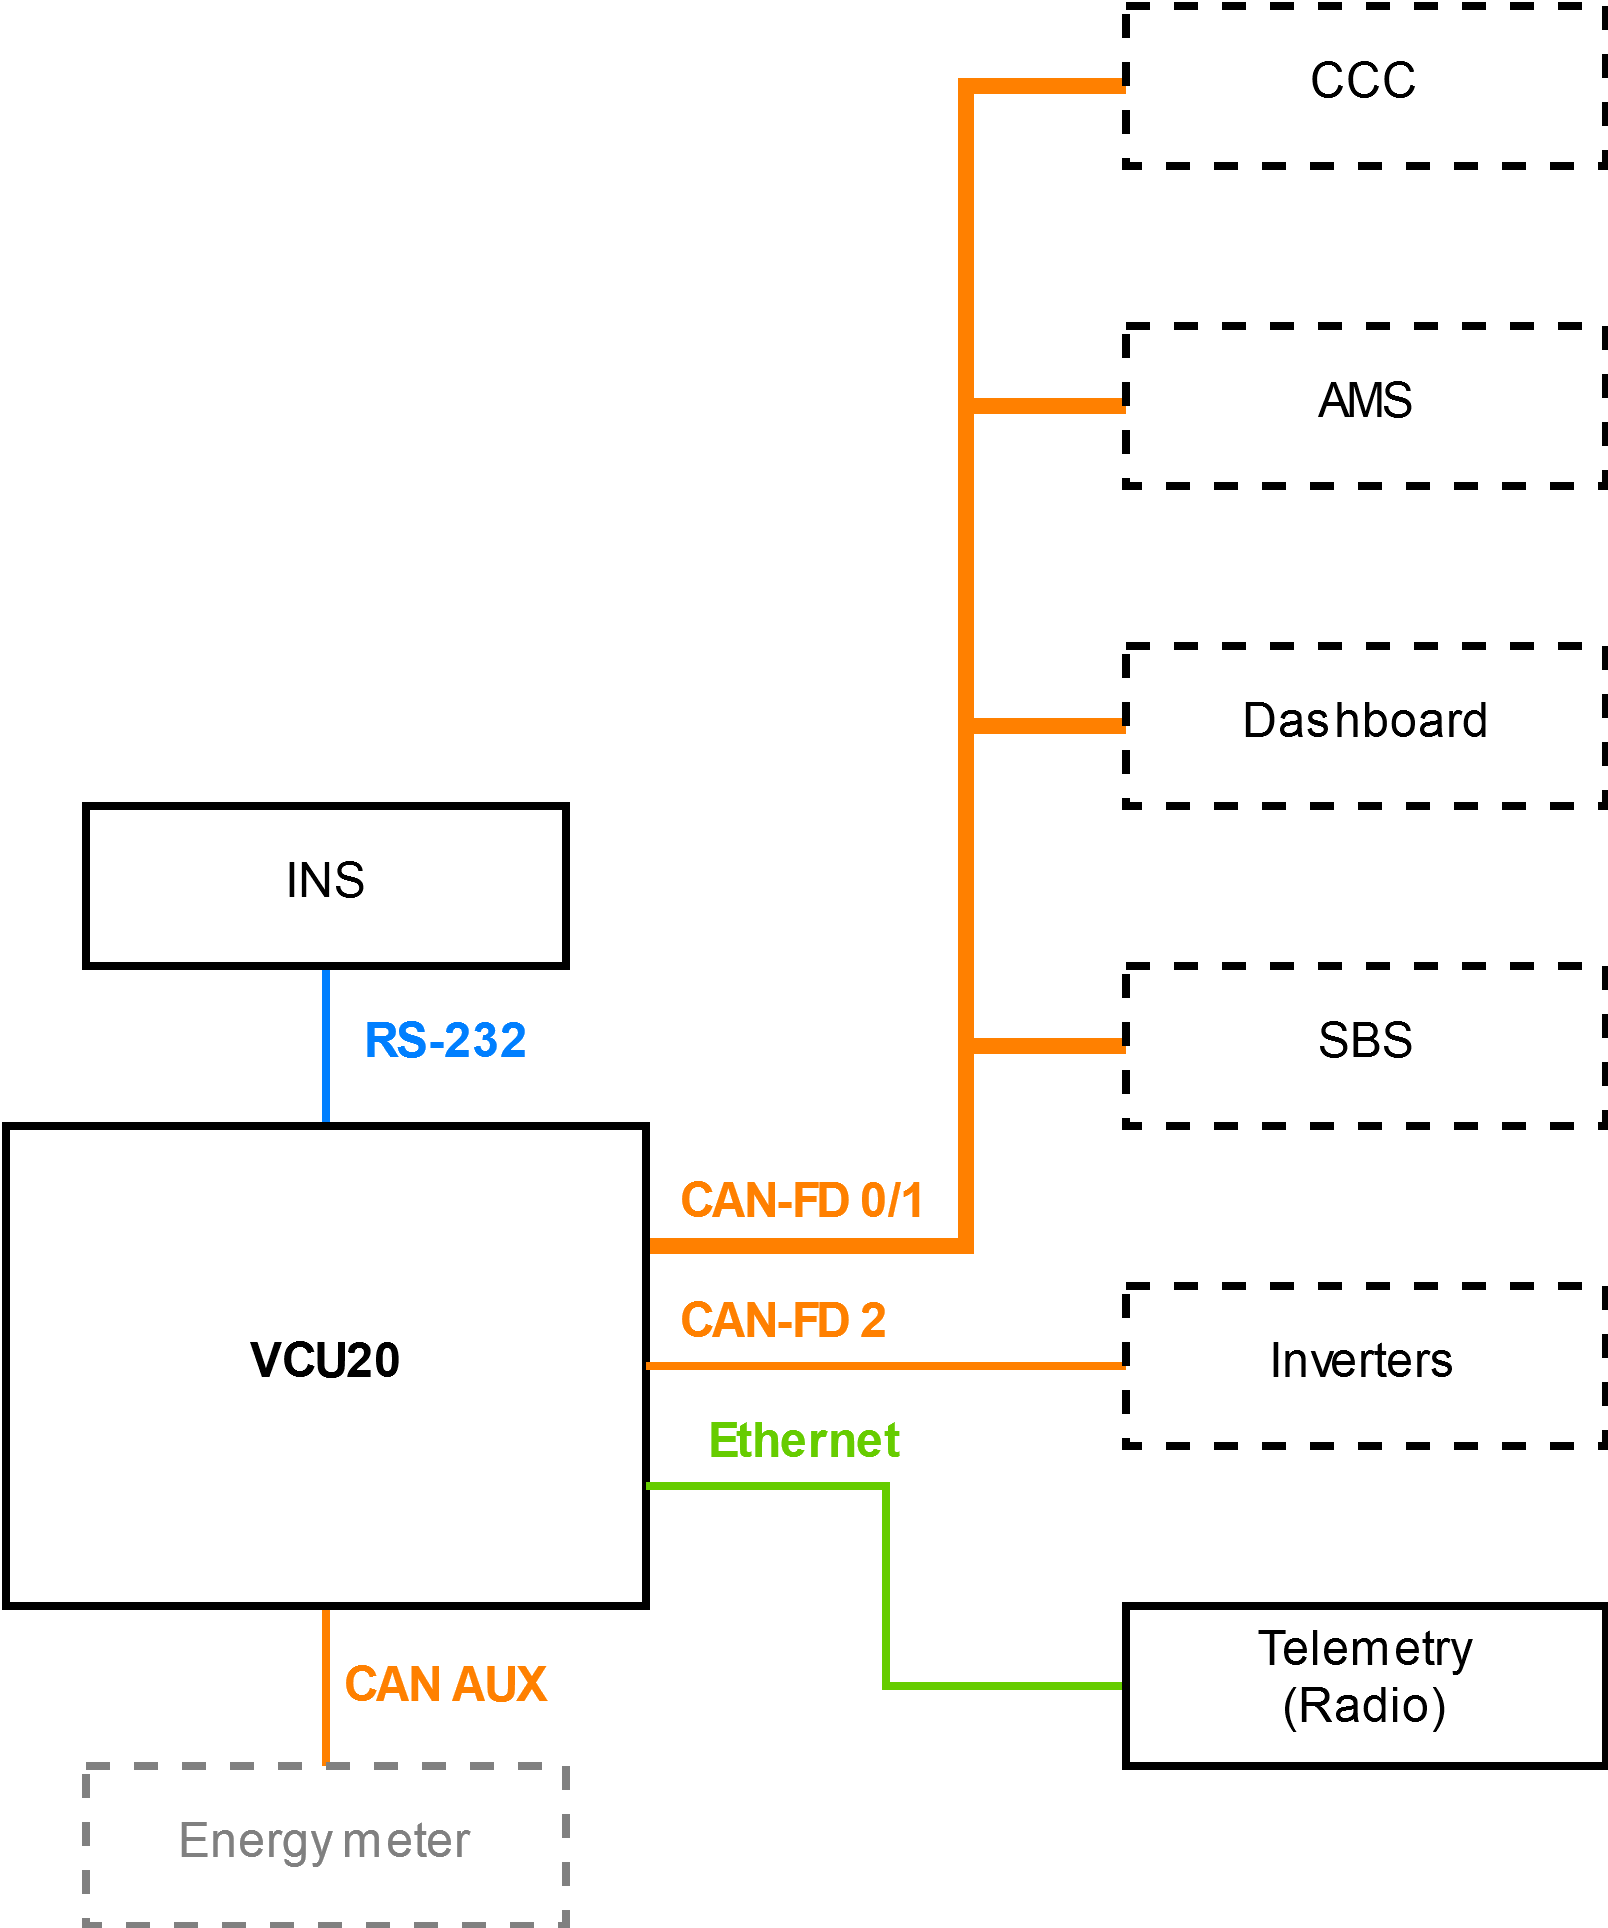
\includegraphics[width=.65\textwidth]{media/vcu20_system.png}
    \caption{Author's \acrshort{vcu20} interface overview. Main focus on communication interfaces.}
    \label{fig:vcu20_system}
\end{figure}

% Looking at the messages which are being transmitted be the telemetry system, it is evident that much of the data originates from the VCU. However, most of this data does not need to be read by any other embedded system on the vehicle. A great improvement from last seasons design would therefore be to add an Ethernet interface to the VCU. This should reduce the load on the bus by a lot.
